%Signal quality assessment is a fundamental component in the area of health monitoring applications, especially in the context of health applications in wearable devices%~\cite{lucafo2022}. These wearable devices serve as instruments for the continuous measurement of vital signs and health parameters, yet their efficacy is contingent upon the rigorous evaluation of the signals they capture. Although those devices are usually designed for long periods of monitoring, they use an optical method to obtain a \acrfull{ppg}, signal type that may deteriorate due to many factors, including motion artifacts or changes in illumination, thereby requiring signal quality assessment mechanisms to check its reliability. The quality of the data derived from these devices plays a decisive function in the efficacy of machine learning and artificial intelligence algorithms, frequently deployed for health data analysis and decision-making. Thus, by ensuring signal quality, wearable health applications can mitigate false alarms, deliver tailored healthcare recommendations, bolster research endeavors, and enhance device adoption and long-term utilization, consequently advancing the landscape of healthcare and patient well-being. In this work, we propose a solution for the problem of assessing the quality of 1D %\acrshort{ppg} signals by projecting them into 2D images, to take advantage of %\gls{CV} techniques, which requires bi-dimensional data.

The human civilization constantly seeks improvements in life longevity and quality. One of the main research areas in that regard is the medicine, which provides means of preventing and remedying accidents and diseases. Diseases, specifically, can deteriorate a person's health silently. An example of that is the presence of atheromas, which, when untreated, can lead to lethal events such as heart attacks and strokes. For that reason, it is important to periodically search professional medical advice to detect diseases at early stages when it is still easy to treat them. However, individual professional service is expensive for most people and is unresponsive to sudden changes. Therefore, there is a demand for an automatic and constant health monitoring method.  

A promising solution for that demand is the remote healthcare. That approach is only possible with the advent of the \gls{IoT}, which is, in concept, a scalable network of interconnected devices that exchange information possibly acquired by sensors. That is interesting to healthcare when those sensors extract environmental and physiological data that can hint the patient conditions. Examples of such data are body temperature, blood pressure and neural activity. We can obtain those indicators in the patient daily life through wearable devices that resemble quotidian objects, with the shape of belts, bracelets, rings, shoe soles, clothing, etc. An popular example of such wearables is the smart watch which, similarly to smartphones, can execute tasks unusual to a simple watch as, with healthcare in mind, recording \gls{PPG} data. Since devices like those support wireless connection, they can send that data to either directly to a medical staff or, as the now popular big data trend promotes, to an automatic intelligent system in the cloud. That intelligent system can, among countless patients, choose special cases that need attention. Therefore, the remote healthcare promises easier than ever access to key physiological signal data.  

However, the extraction of physiological signals such as the \gls{PPG} is not free of interferences. The \gls{PPG}, for example, is under the influence of changes in illumination, low sensor quality, the user skin physiognomy, the sensor positioning, etc. But the main sources of interference are motion artifacts, which can cause high-amplitude distortions that not only can destroy the core information but also can produce misleading events. That is unacceptable in healthcare applications, since misdiagnosis can expose the healthy patient to unnecessary risk, while lack of diagnosis can leave the unhealthy patient unattended. For that reason, it is of extreme importance to verify the quality of the signal before proceeding to further analysis on the signal. That task is known as \gls{SQA} and this thesis proposes a method to achieve that goal for \gls{PPG} signals.    

\section{Photopletysmograph signal}

\gls{PPG} signals are, in essence, optical signals that results from the light interaction with the human tissues. To extract the signal, we need two basic components. The first is a light source, to emit light towards the tissues. An example of light source is the \gls{LED}. The second is a light receptor, to measure the light intensity. For that, we can use a photodiode, but there are attemps of using cameras. To prepare the signal extraction, we need to place those two type of devices exploiting one of two light interaction principles. The figure \ref{fig:method:ppg} shows both of them. One of them is the human tissue reflectance, that is, the property of the human tissues reflecting the incoming light rays. In that case, we need to place the devices in such manner that the human tissues are not between them. An example of application are the smartwatches, since all devices are bellow the main structure.  The other principle is the human tissue permeability, that is, the property of the light being able to traverse the human tissues. In that second case, the device placement is the negative of the first, that is, the human tissues need to be between the devices. An example of that case are fingertip pulse oximeters. At this point, the set up is ready to extract the \gls{PPG} signal.

\begin{figure}[h!]
	\centering
	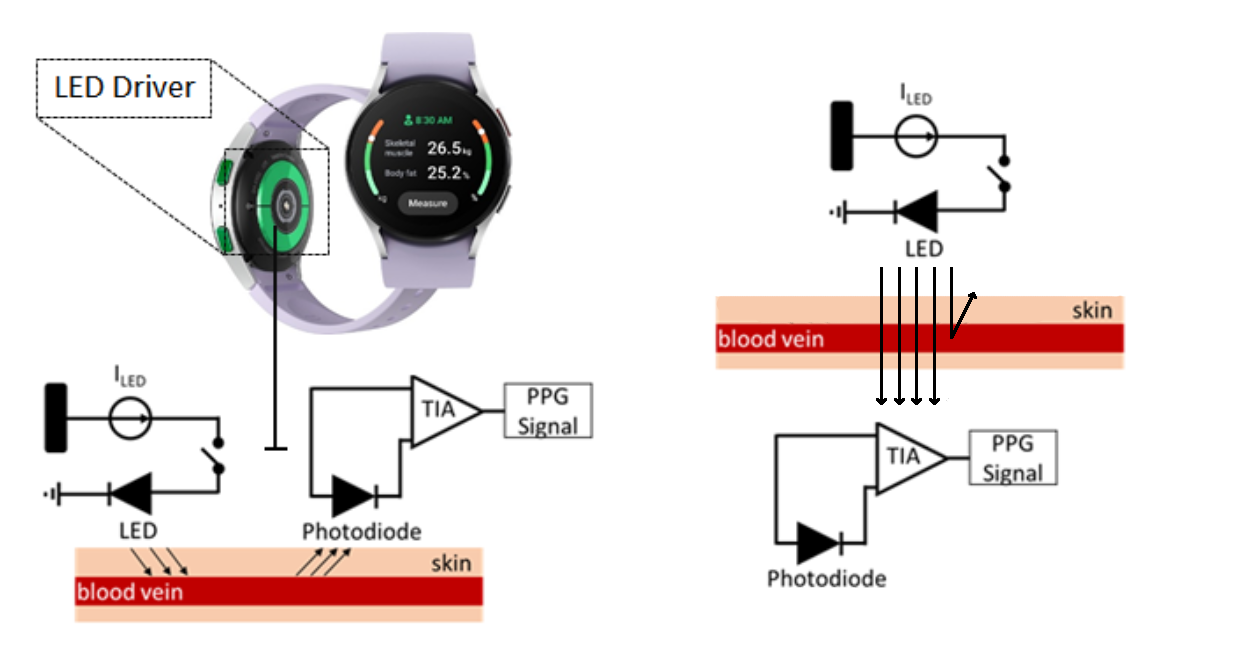
\includegraphics[width=0.9\textwidth]{img/ppg.png}
	\caption{Schematic illustration of a \gls{PPG} sensor. On the left, the signal is obtained through the reflectivity of light by human tissue, while on the right, it is obtained through the permeability of light through human tissue. This figure is a courtesy of Lucafó et al.~\protect\cite{deep-learning-3}}
	\label{fig:method:ppg}
\end{figure}

